\documentclass[12pt]{article}
\usepackage[top=1in,left=1in, right = 1in, footskip=1in]{geometry}

\usepackage{graphicx}
\usepackage{xspace}
%\usepackage{adjustbox}

\newcommand{\comment}{\showcomment}
%% \newcommand{\comment}{\nocomment}

\newcommand{\showcomment}[3]{\textcolor{#1}{\textbf{[#2: }\textsl{#3}\textbf{]}}}
\newcommand{\nocomment}[3]{}

\newcommand{\jd}[1]{\comment{cyan}{JD}{#1}}
\newcommand{\swp}[1]{\comment{magenta}{SWP}{#1}}
\newcommand{\bmb}[1]{\comment{blue}{BMB}{#1}}
\newcommand{\djde}[1]{\comment{red}{DJDE}{#1}}

\newcommand{\eref}[1]{Eq.~\ref{eq:#1}}
\newcommand{\fref}[1]{Fig.~\ref{fig:#1}}
\newcommand{\Fref}[1]{Fig.~\ref{fig:#1}}
\newcommand{\sref}[1]{Sec.~\ref{#1}}
\newcommand{\frange}[2]{Fig.~\ref{fig:#1}--\ref{fig:#2}}
\newcommand{\tref}[1]{Table~\ref{tab:#1}}
\newcommand{\tlab}[1]{\label{tab:#1}}
\newcommand{\pday}{\ensuremath{/\textrm{day}}}

\usepackage{amsthm}
\usepackage{amsmath}
\usepackage{amssymb}
\usepackage{amsfonts}

\usepackage{lineno}
\linenumbers

\usepackage[pdfencoding=auto, psdextra]{hyperref}

\usepackage{natbib}
\bibliographystyle{chicago}
\date{\today}

\usepackage{xspace}
\newcommand*{\ie}{i.e.\@\xspace}

\usepackage{color}

\newcommand{\Rx}[1]{\ensuremath{{\mathcal R}_{#1}}\xspace} 
\newcommand{\Ro}{\Rx{0}}
\newcommand{\Rc}{\Rx{\mathrm{c}}}
\newcommand{\Ri}{\Rx{\mathrm{i}}}
\newcommand{\RR}{\ensuremath{{\mathcal R}}\xspace}
\newcommand{\Rhat}{\ensuremath{{\hat\RR}}}
\newcommand{\Rprop}{\Rx{\mathrm{prop}}}
\newcommand{\Rcori}{\Rx{\mathrm{cori}}}
\newcommand{\tsub}[2]{#1_{{\textrm{\tiny #2}}}}
\newcommand{\dd}[1]{\ensuremath{\, \mathrm{d}#1}}
\newcommand{\dtau}{\dd{\tau}}
\newcommand{\dx}{\dd{x}}
\newcommand{\dsigma}{\dd{\sigma}}

\newcommand{\tstart}{\ensuremath{\tsub{t}{start}}\xspace}
\newcommand{\tend}{\ensuremath{\tsub{t}{end}}\xspace}

\newcommand{\betaeff}{\ensuremath{\tsub{\beta}{eff}}\xspace}
\newcommand{\Keff}{\ensuremath{\tsub{K}{eff}}\xspace}
\newcommand{\Kpost}{\ensuremath{\tsub{K}{post}}\xspace}

\newcommand{\pt}{p} %% primary time
\newcommand{\st}{s} %% secondary time

\newcommand{\psize}{{\mathcal P}} %% primary cohort size
\newcommand{\ssize}{{\mathcal S}} %% secondary cohort size

\newcommand{\gtime}{\sigma} %% generation interval
\newcommand{\gdist}{g} %% generation-interval distribution

\newcommand{\geff}{g_{\textrm{eff}}} %% generation-interval distribution

\newcommand{\total}{{\mathcal T}} %% total number of serial intervals

\newcommand{\PP}{\ensuremath{\mathcal P}}
\newcommand{\II}{\ensuremath{\mathcal I}}
\newcommand{\HH}{\ensuremath{\mathcal H}}

\begin{document}

\begin{flushleft}{
	\Large
	\textbf\newline{
		Immune boosting bridges leaky vaccine and polarized vaccine models
	}
}
\newline
\\
Sang Woo Park\textsuperscript{1,*}, Chadi Saad-Roy, ???, Jessica Metcalf, Bryan T Grenfell, Jonathan Dushoff
\\
\bigskip
\textbf{1} Department of Ecology and Evolutionary Biology, Princeton University, Princeton, NJ, USA
\\
\bigskip

*Corresponding author: swp2@princeton.edu
\end{flushleft}

In this study, we compare different models of immunity.
First, we illustrate that the difference between the standard (``leaky'') immunity model and the polarized immunity models can be reconciled via immune boosting mechanism.



\section{Mathematical models of vaccine-induced immunity}

\begin{figure}[!tp]
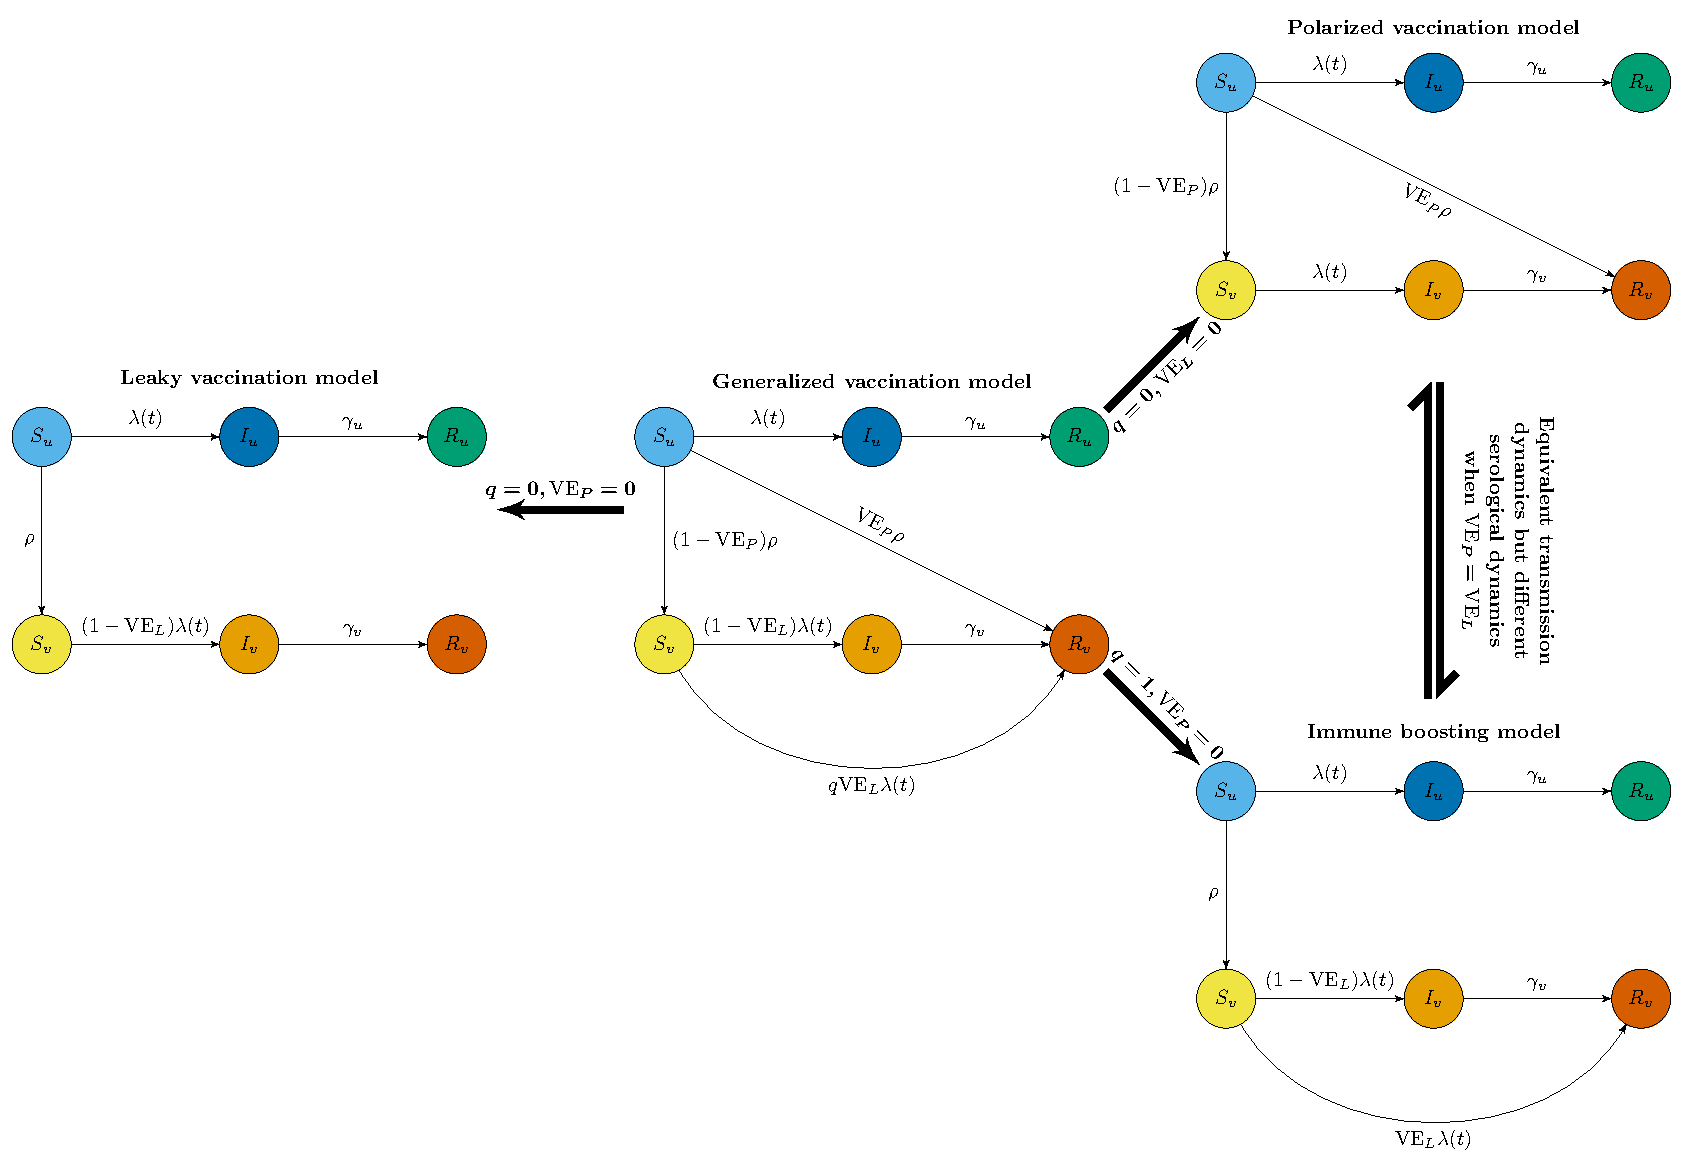
\includegraphics[width=\textwidth]{figure_diagram_comb.pdf}
\caption{
\textbf{A schematic diagram of vaccine models}
}
\end{figure}

First, we begin with a standard SIR model with a leaky vaccine, in which all vaccinated individuals experience a reduced force of infection by a factor of $p$:
\begin{align}
\frac{\dd S}{\dd t} &= - \lambda(t) S - \rho S \\
\frac{\dd I_u}{\dd t} &= \lambda(t) S - \gamma_u I_u \\
\frac{\dd R_u}{\dd t} &= \gamma_u I_u \\
\frac{\dd V}{\dd t} &= - p \lambda(t) V + \rho S \\
\frac{\dd I_v}{\dd t} &= p \lambda(t) V - \gamma_v I_v \\
\frac{\dd R_v}{\dd t} &= \gamma_v I_v
\end{align}
where $\lambda$ represents the baseline force of infection experienced by unvaccinated individuals; $\rho$ represents vaccination rate; and $\gamma_u$ and $\gamma_v $ represent the recovery of the unvaccinated and vaccinated individuals, respectively.
This kind of model is also referred to as a history-based model as the susceptibility of an individual depends on the history of infections or vaccination---in this case, all individuals who have the same vaccine history have identical susceptibility.

On the other hand, the polarized vaccination model assumes that a proportion $p$ of vaccinated individuals still remain susceptible, whereas the remaining proportion $1-p$ become fully immune: 
\begin{align}
\frac{\dd S}{\dd t} &= - \lambda(t) S - \rho S \\
\frac{\dd I_u}{\dd t} &= \lambda(t) S - \gamma_u I_u \\
\frac{\dd R_u}{\dd t} &= \gamma_u I_u \\
\frac{\dd V}{\dd t} &= - \lambda(t) V + p \rho S \\
\frac{\dd I_v}{\dd t} &= \lambda(t) V - \gamma_v I_v \\
\frac{\dd R_v}{\dd t} &= \gamma_v I_v + (1-p) \rho S
\end{align}
The polarized immunity model is often used in status-based models for cross immunity---the status-based models keep track of immune statuses of individuals, rather than their infection histories.

While both the standard vaccination model and the polarized vaccination model have been widely used in literature, their assumptions lead to a key dynamical differences: the standard vaccination model assumes that all vaccinated individuals can be eventually infected, whereas the polarized vaccination model assumes that proportion $1-p$ of vaccinated individuals will never be infected.
In other words, the polarized vaccination model will always predict a lower final size than the standard vaccination model.

To better understand these differeces, we consider a immune boosting model.
The standard vaccination model assumes that vaccinated individuals have an independent probability $p$ of infection for every challenge and will otherwise remain partially susceptible.
Instead, the immune boosting model assumes that unsuccessful challenges elicit immune response, moving individuals from $V$ to $R_v$ compartment at rate $(1-p) \lambda(t)$ and thereby breaking the independence assumption: 
\begin{align}
\frac{\dd S}{\dd t} &= - \lambda(t) S - \rho S \\
\frac{\dd I_u}{\dd t} &= \lambda(t) S - \gamma_u I_u \\
\frac{\dd R_u}{\dd t} &= \gamma_u I_u \\
\frac{\dd V}{\dd t} &= - \lambda(t) V + \rho S \\
\frac{\dd I_v}{\dd t} &= p \lambda(t) V - \gamma_v I_v \\
\frac{\dd R_v}{\dd t} &= (1-p) \lambda(t) V + \gamma_v I_v
\end{align}
In this model, both unvaccinated and vaccinated individuals are subject to identical forces of infections, which represent the per capita rate of challenges, but the outcome of challenges differ.
Since the depletion of vaccinated population $V$ always occurs at a faster rate under the immune boosting model than under the standard vaccination model, the immune boosting model always predicts a lower final size.
Furthermore, epidemiological dynamics (i.e., trajectories of $I_u$ and $I_v$) predicted by the immune boosting model and the polarized vaccination model are identical: 
both models assume that individuals become vaccinated at rate $\rho$ and move out of the $V$ compartment at rate $\lambda$ and only differ in when individuals get sorted.
Such equivalence allows us to bridge the difference between the standard and polarized vaccination models.
We note that this equivalence does not hold when immunity wanes as we show later.

While both models predict equivalent epidemic dynamics, they differ in their serological dynamics.

Finally, we present a generalized vaccination model that encompasses all three models:
\begin{align}
\frac{\dd S}{\dd t} &= - \lambda(t) S - \rho S \\
\frac{\dd I_u}{\dd t} &= \lambda(t) S - \gamma_u I_u \\
\frac{\dd R_u}{\dd t} &= \gamma_u I_u \\
\frac{\dd V}{\dd t} &= - \lambda(t) V + \rho S \\
\frac{\dd I_v}{\dd t} &= p \lambda(t) V - \gamma_v I_v \\
\frac{\dd R_v}{\dd t} &= (1-p) \lambda(t) V + \gamma_v I_v
\end{align}



\begin{figure}[!tp]
\includegraphics[width=\textwidth]{figure_simulation_generalized.pdf}
\caption{
\textbf{A schematic diagram of vaccine models}
}
\end{figure}

 

\end{document}
